\documentclass[UTF8]{ctexart}
\usepackage[a4paper,margin=2.2cm]{geometry}
\usepackage{graphicx}
\usepackage{booktabs}
\usepackage{tabularx}
\usepackage{subcaption}
\usepackage{float}
\usepackage{placeins}
\usepackage{array}

% 混淆矩阵子图高度（与汇总表同页时需偏紧，可按编译效果微调 0.10--0.13）
\newcommand{\cmfig}[1]{\includegraphics[width=\linewidth,height=0.115\textheight,keepaspectratio]{#1}}

\begin{document}

% --- 封面 ---
\begin{titlepage}
  \begin{center}
    \vspace*{2.8cm}
    {\Huge \songti \textbf{STL10 图像分类模型优化实验报告}}\par
    \vspace{0.45cm}
    {\Large \songti 人工智能原理课程 · 项目二 · STL10 图像分类}\par

    \vspace{5.5cm}

    {\large
    \renewcommand{\arraystretch}{2}
    \begin{tabular}{r c}
      \makebox[2.5cm][s]{院 系}：& \makebox[6cm][c]{自动化系} \\ \cline{2-2}
      \makebox[2.5cm][s]{班 级}：& \makebox[6cm][c]{自52班} \\ \cline{2-2}
      \makebox[2.5cm][s]{学生姓名}：& \makebox[6cm][c]{刘江宇} \\ \cline{2-2}
      \makebox[2.5cm][s]{学 号}：& \makebox[6cm][c]{2024013215} \\ \cline{2-2}
      \makebox[2.5cm][s]{课程名称}：& \makebox[6cm][c]{人工智能原理} \\ \cline{2-2}
    \end{tabular}
    }
  \end{center}
\end{titlepage}

\newpage

\tableofcontents
\newpage

\section{实验目标}
基于 baseline CNN，在 STL10 数据集上开展优化实验，尝试在模型训练过程当中可能会影响模型效果的因素，更好地掌握上课学习到的内容
重点比较不同因素对模型效果的影响，包括：
\begin{itemize}
  \item 数据增强是否提升泛化能力；
  \item BatchNorm 与 Dropout 对收敛和过拟合的影响；
  \item 优化器与学习率设置对最终测试表现的影响；
  \item 更深网络（\texttt{improved\_long}，多段池化）相对浅层 configurable 的收益。
\end{itemize}
同时还通过Grad-CAM进行可解释性的分析，更好地理解模型为什么能够做出这样的预测

\section{实验设置}
\begin{itemize}
  \item 数据来源：\texttt{STL10/train} 与 \texttt{STL10/test}。（课程提供）
  \item 训练配置：固定 \texttt{epochs=50}、\texttt{batch\_size=128}、\texttt{val\_ratio=0.1}、\texttt{seed=42}。
  \item 评估指标：Accuracy、Macro-F1、Weighted-F1、分类报告、混淆矩阵。
  \item 输出目录：\texttt{outputs\_improved/}。（可在压缩包或github上查看）
\end{itemize}

\section{实验分组}
实验主要有8组，分别在baseline的基础上进行修改，包括数据增强、BatchNorm、Dropout、优化器、学习率、网络深度等
\begin{itemize}
  \item baseline：基础 CNN，无增强、无 BN、无 Dropout（Adam, lr=0.001, L2 \texttt{weight\_decay=5e-4}）
  \item exp1\_aug：数据增强（RandomCrop + HorizontalFlip + ColorJitter）
  \item exp2\_aug\_bn：数据增强 + BatchNorm
  \item exp3\_aug\_dropout：数据增强 + Dropout(0.3)
  \item exp4\_aug\_bn\_sgd：与 exp2 相同（增强 + BN、无 Dropout），优化器改为 SGD（\texttt{lr=0.01}）
  \item exp5\_aug\_bn\_lr：与 exp2 相同，Adam 学习率改为 \texttt{3e-4}
  \item exp6\_improved\_long\_6：与 exp2 相同，卷积层数改为6
  \item exp7\_improved\_long\_9：与 exp2 相同，卷积层数改为9
  \item exp8\_improved\_longer\_12：与 exp2 相同，卷积层数改为12
\end{itemize}

\clearpage
\section{实验结果概览}
下面附上全部实验的实验结果，其中test成功率最低的为baseline，为54.70\%，最高的为exp7\_improved\_long\_9，为81.60\%。
详细的训练分析在后面会给出
\begin{center}
\begin{minipage}[t]{0.95\textwidth}
\centering
\footnotesize
\noindent\resizebox{\linewidth}{!}{%
\begin{tabular}{@{}lcccc@{}}
\toprule
实验组 & Best Val Acc(\%) & Test Acc(\%) & Macro-F1 & Weighted-F1 \\
\midrule
baseline & 61.43 & 54.70 & 0.5464 & 0.5464 \\
exp1\_aug & 71.57 & 66.50 & 0.6688 & 0.6688 \\
exp2\_aug\_bn & 77.14 & 71.70 & 0.7178 & 0.7178 \\
exp3\_aug\_dropout & 74.14 & 69.00 & 0.6918 & 0.6918 \\
exp4\_aug\_bn\_sgd & 74.57 & 70.30 & 0.7052 & 0.7052 \\
exp5\_aug\_bn\_lr & 74.43 & 69.80 & 0.6959 & 0.6959 \\
exp6\_improved\_long\_6 & 82.71 & 80.40 & 0.8055 & 0.8055 \\
exp7\_improved\_long\_9 & 81.57 & \textbf{81.60} & \textbf{0.8153} & \textbf{0.8153} \\
exp8\_improved\_longer\_12 & 70.29 & 69.50 & 0.6948 & 0.6948 \\
\bottomrule
\end{tabular}%
}
\captionof{table}{各实验组性能对比（见 \texttt{comparison\_summary.csv}）}
\label{tab:summary}

\vspace{0.45\baselineskip}

\captionsetup{type=figure}
\setlength{\abovecaptionskip}{2pt}
\begin{tabularx}{\linewidth}{@{}>{\centering\arraybackslash}X>{\centering\arraybackslash}X>{\centering\arraybackslash}X@{}}
\cmfig{../outputs_improved/baseline/figures/baseline_baseline_confusion_matrix.png} &
\cmfig{../outputs_improved/exp1_aug/figures/exp1_aug_baseline_confusion_matrix.png} &
\cmfig{../outputs_improved/exp2_aug_bn/figures/exp2_aug_bn_configurable_confusion_matrix.png} \\
\scriptsize baseline &
\scriptsize exp1\_aug &
\scriptsize exp2\_aug\_bn \\
\addlinespace[2pt]
\cmfig{../outputs_improved/exp3_aug_dropout/figures/exp3_aug_dropout_configurable_confusion_matrix.png} &
\cmfig{../outputs_improved/exp4_aug_bn_sgd/figures/exp4_aug_bn_sgd_configurable_confusion_matrix.png} &
\cmfig{../outputs_improved/exp5_aug_bn_lr/figures/exp5_aug_bn_lr_configurable_confusion_matrix.png} \\
\scriptsize exp3\_aug\_dropout &
\scriptsize exp4\_aug\_bn\_sgd &
\scriptsize exp5\_aug\_bn\_lr \\
\addlinespace[2pt]
\cmfig{../outputs_improved/exp6_improved_long_6/figures/exp6_improved_long_6_improved_long_confusion_matrix.png} &
\cmfig{../outputs_improved/exp7_improved_long_9/figures/exp7_improved_long_9_improved_longer_confusion_matrix.png} &
\cmfig{../outputs_improved/exp8_improved_longer_12/figures/exp8_improved_longer_12_improved_longer_12_confusion_matrix.png} \\
\scriptsize exp6\_improved\_long\_6 &
\scriptsize exp7\_improved\_long\_9 &
\scriptsize exp8\_improved\_longer\_12 \\
\end{tabularx}
\captionof{figure}{测试集混淆矩阵（$3\times3$）}
\label{fig:cm_all}
\end{minipage}
\end{center}
\FloatBarrier

\section{训练过程与结果分析}
\noindent 下面按对照分组放了训练曲线：每张图从左到右是训练/验证的 loss 和准确率，虚线是参照组、实线是对照组。数字以表~\ref{tab:summary} 为准，图主要是看收敛快慢和 train、val 差得大不大。

\subsection{（一）baseline $\rightarrow$ exp1：数据增强}
\begin{itemize}
  \item baseline 测试只有 54.70\%，exp1 拉到 66.50\%，成功率提升很多
  \item 从曲线上看，baseline的过拟合非常严重，exp1的过拟合程度明显减轻，说明数据增强确实有效果
\end{itemize}
\begin{figure}[H]
  \centering
  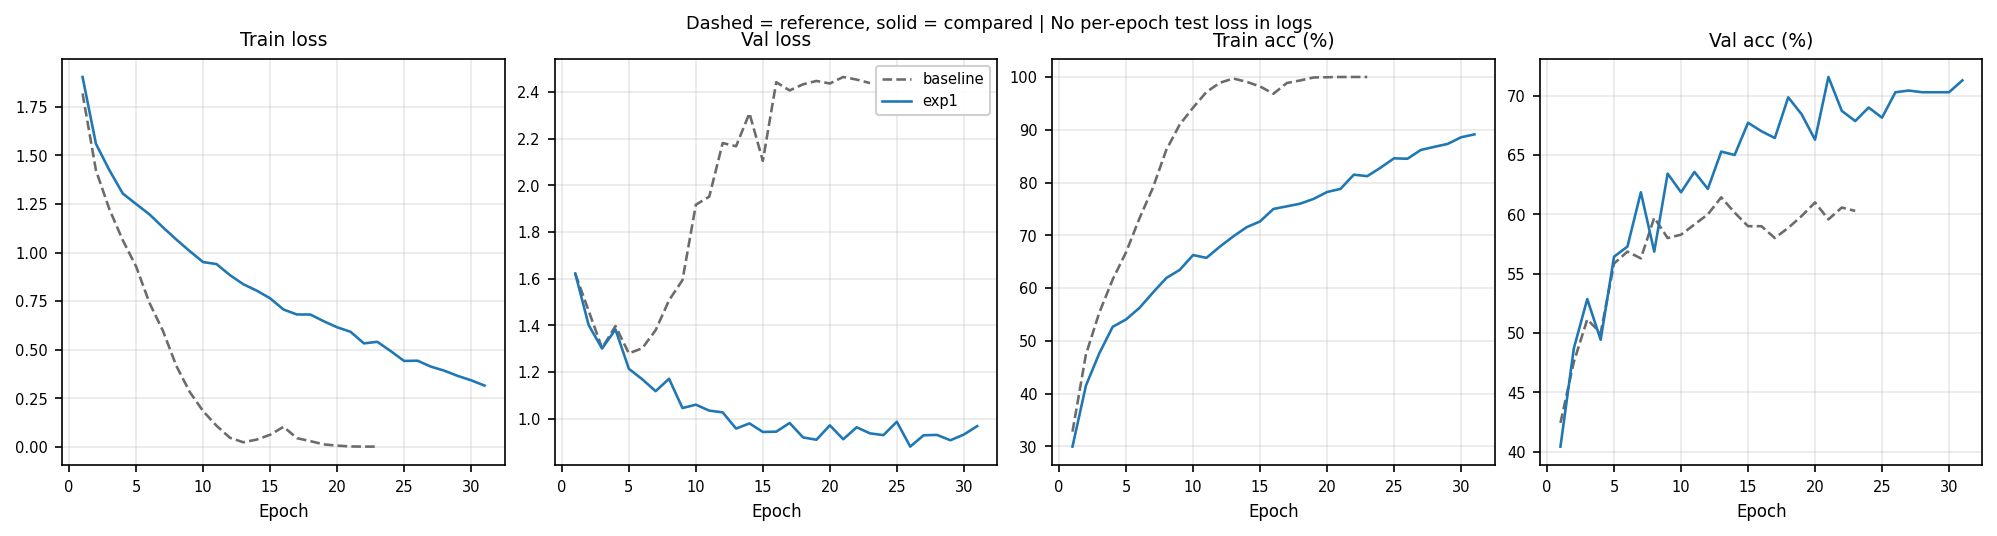
\includegraphics[width=\linewidth]{figures/comparisons/cmp_01_baseline_exp1.png}
  \caption{baseline（虚线）与 exp1\_aug（实线）：训练/验证 loss 与准确率}
\end{figure}

\subsection{（二）exp1 $\rightarrow$ exp2：BatchNorm}
\begin{itemize}
  \item exp1 测试 66.50\%，exp2 到 71.70\%，又涨了 5 个点左右，说明在已经有增强的前提下，加上 BN 还是有效减小了过拟合。
\end{itemize}
\begin{figure}[H]
  \centering
  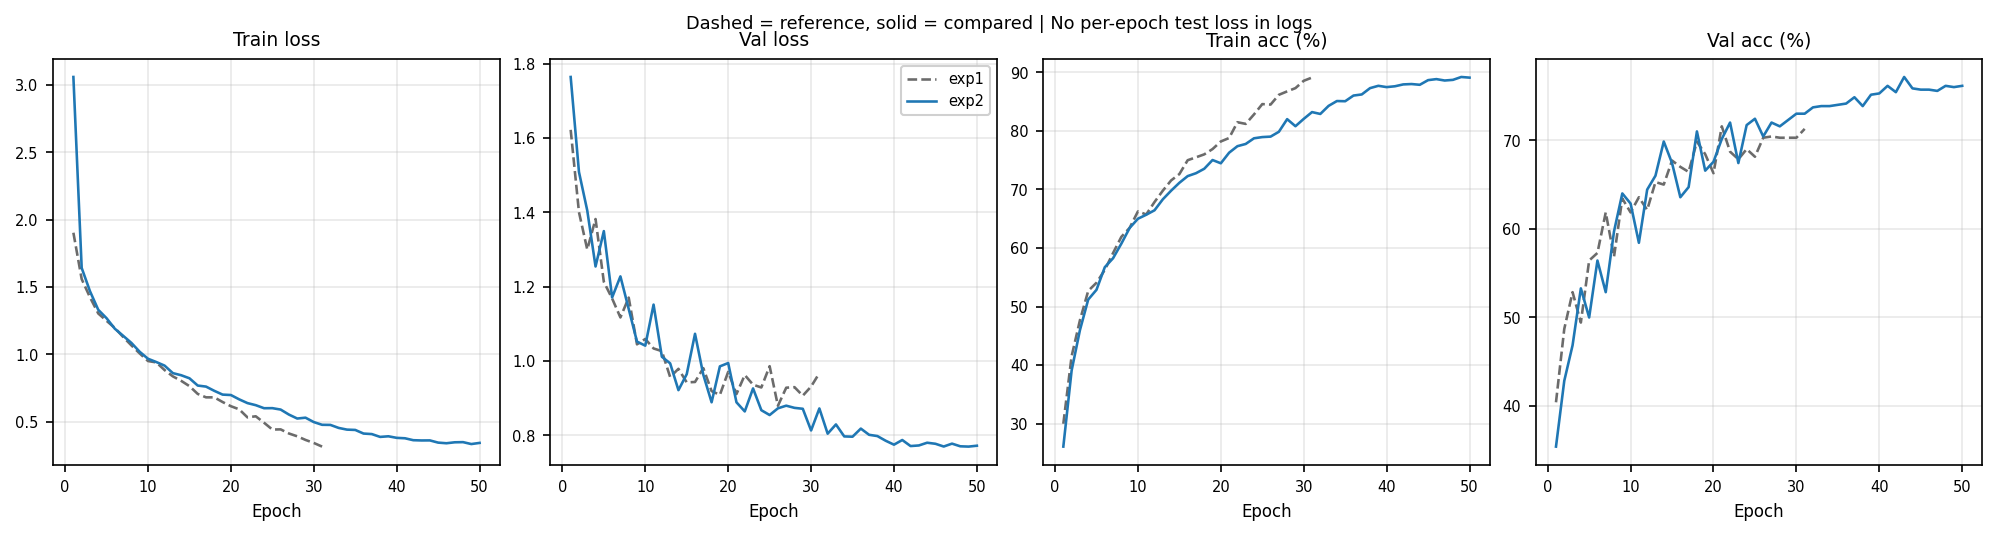
\includegraphics[width=\linewidth]{figures/comparisons/cmp_02_exp1_exp2.png}
  \caption{exp1\_aug（虚线）与 exp2\_aug\_bn（实线）}
\end{figure}

\subsection{（三）exp2 $\rightarrow$ exp3：Dropout（与 BN 路径对照）}
\begin{itemize}
  \item exp2 测试 71.70\%，exp3 只有 69.00\%，但都比baseline好。说明两种办法都很有效，且差异并没有很大。
 \end{itemize}
\begin{figure}[H]
  \centering
  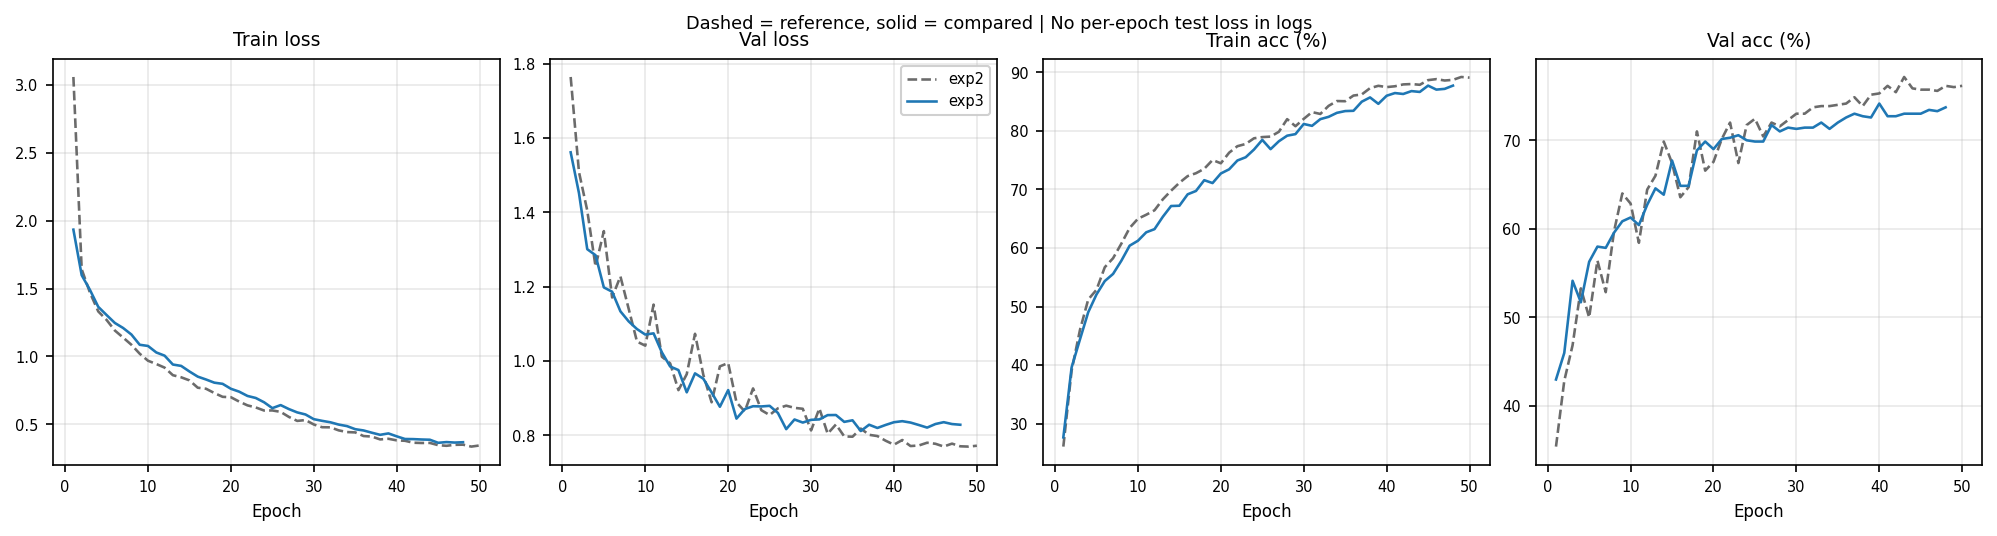
\includegraphics[width=\linewidth]{figures/comparisons/cmp_03_exp2_exp3.png}
  \caption{exp2\_aug\_bn（虚线）与 exp3\_aug\_dropout（实线）}
\end{figure}

\subsection{（四）exp2 $\rightarrow$ exp4：优化器（Adam vs SGD）}
\begin{itemize}
  \item 不同的优化器对比，exp2（Adam）测试 71.70\%，exp4（SGD）70.30\%，差得不大，但确实是 exp2 略好一点。
\end{itemize}
\begin{figure}[H]
  \centering
  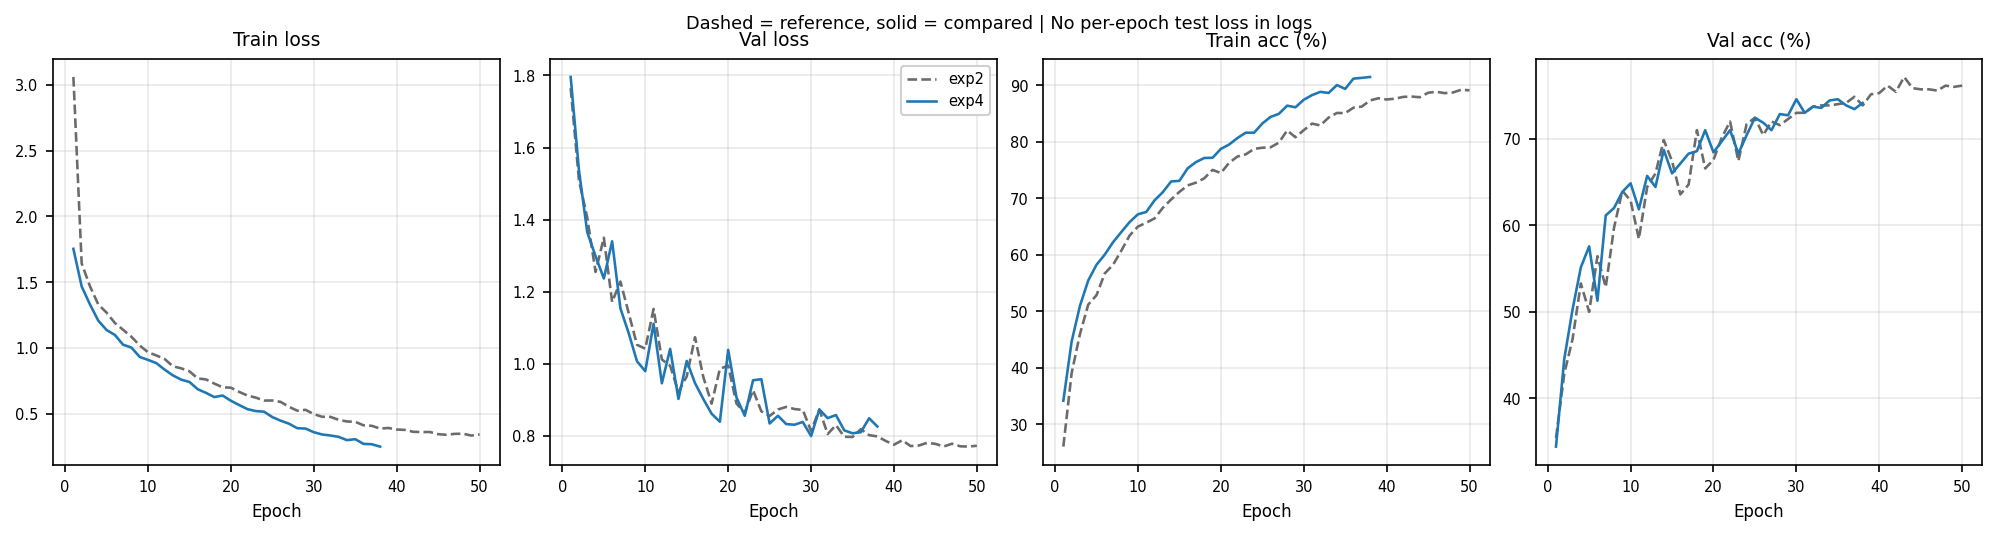
\includegraphics[width=\linewidth]{figures/comparisons/cmp_04_exp2_exp4.png}
  \caption{exp2\_aug\_bn（虚线）与 exp4\_aug\_bn\_sgd（实线）}
\end{figure}

\subsection{（五）exp2 $\rightarrow$ exp5：学习率}
\begin{itemize}
  \item exp2 用 \texttt{1e-3}，exp5 改成 \texttt{3e-4}，测试从 71.70\% 掉到 69.80\% 左右，说明这次并不是学习率越小越稳越好。
\end{itemize}
\begin{figure}[H]
  \centering
  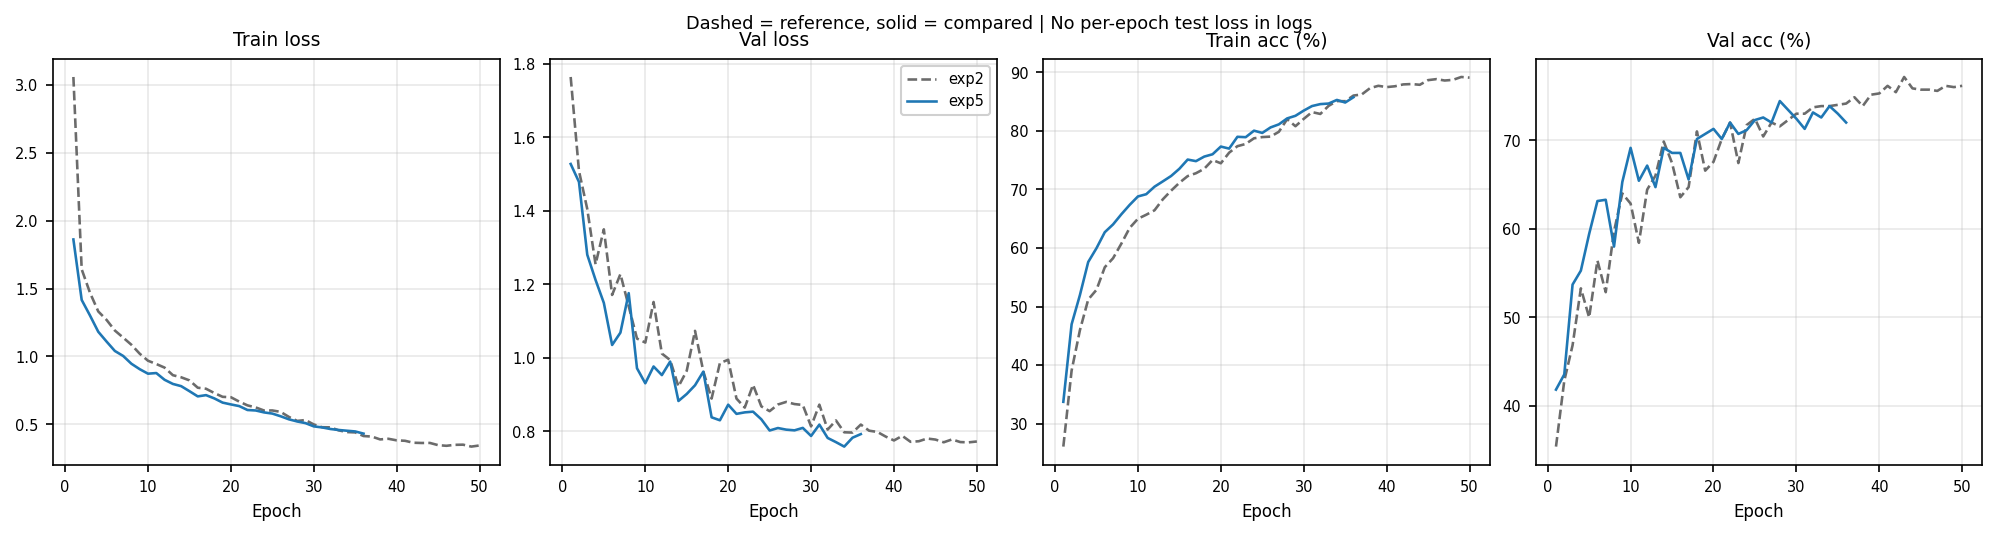
\includegraphics[width=\linewidth]{figures/comparisons/cmp_05_exp2_exp5.png}
  \caption{exp2\_aug\_bn（虚线）与 exp5\_aug\_bn\_lr（实线）}
\end{figure}

\subsection{（六）exp2 $\rightarrow$ exp6 / exp7 / exp8：网络深度}
\begin{itemize}
  \item 浅层 exp2 测试 71.70\%，加深以后 exp6 到 80.40\%、exp7 到 81.60\%（全队最高），说明在一定范围内增加网络深度可以有效提升模型效果。
  \item exp8 又掉到 69.50\%，跟 exp7 差了一大截，说明模型也不是越深越好
\end{itemize}
\begin{figure}[H]
  \centering
  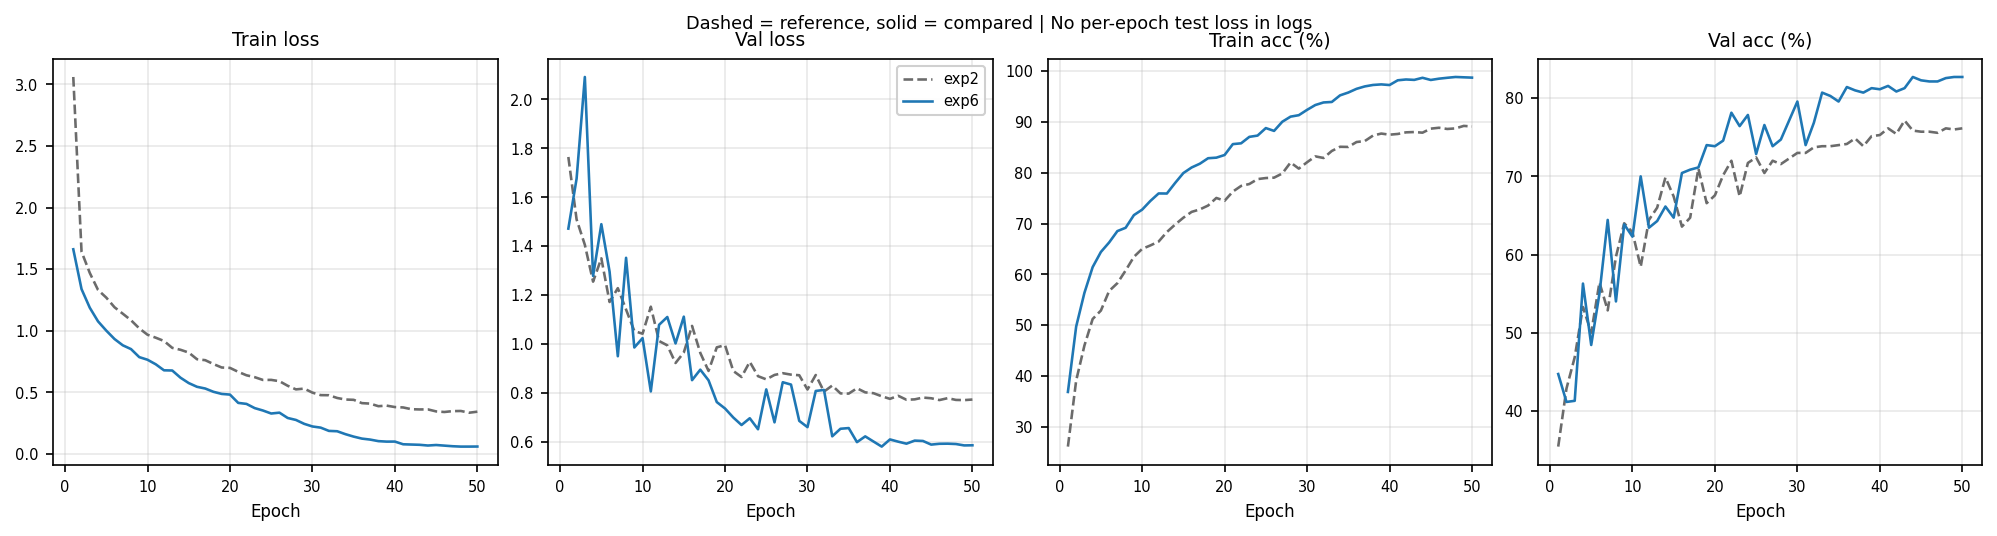
\includegraphics[width=\linewidth]{figures/comparisons/cmp_06a_exp2_exp6.png}
  \caption{exp2\_aug\_bn（虚线）与 exp6\_improved\_long\_6（实线）}
\end{figure}
\begin{figure}[H]
  \centering
  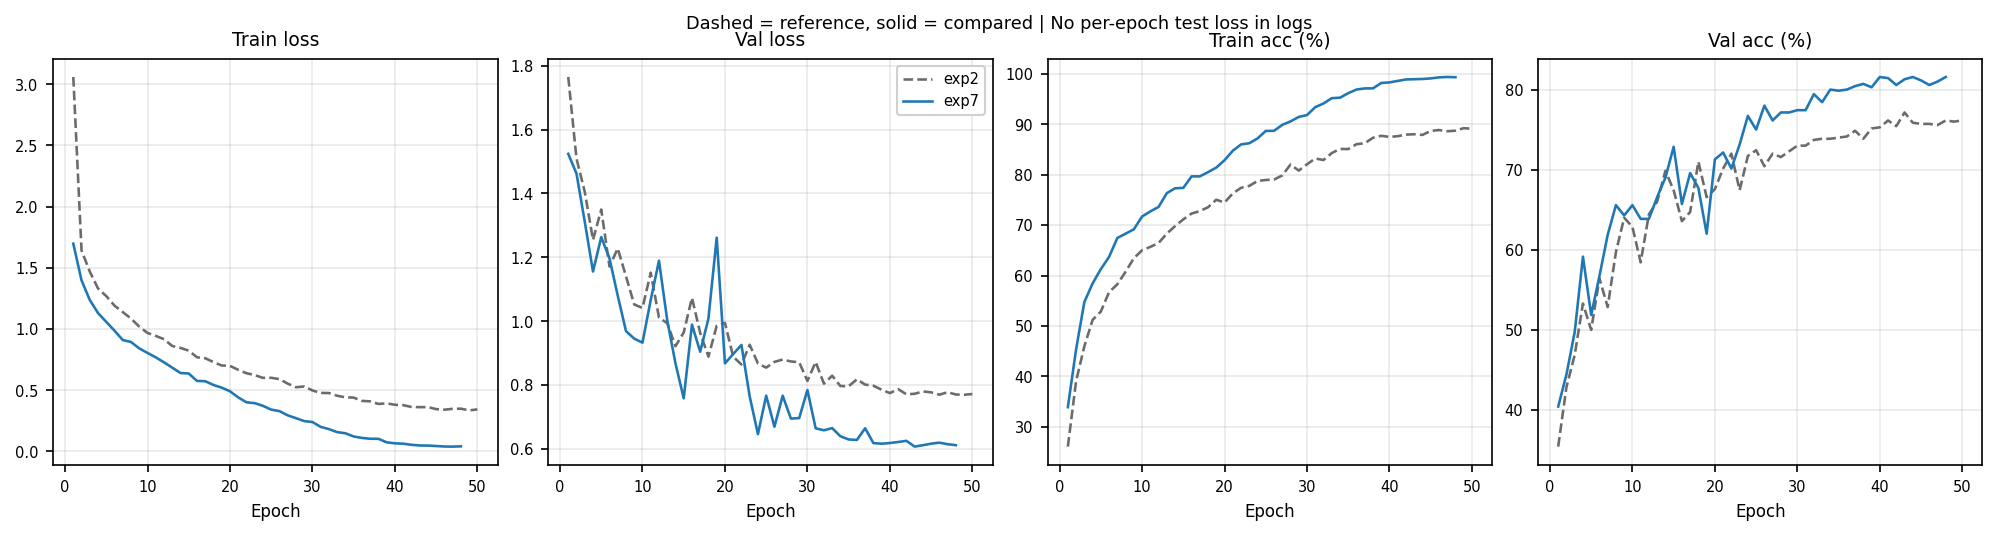
\includegraphics[width=\linewidth]{figures/comparisons/cmp_06b_exp2_exp7.png}
  \caption{exp2\_aug\_bn（虚线）与 exp7\_improved\_long\_9（实线）}
\end{figure}
\begin{figure}[H]
  \centering
  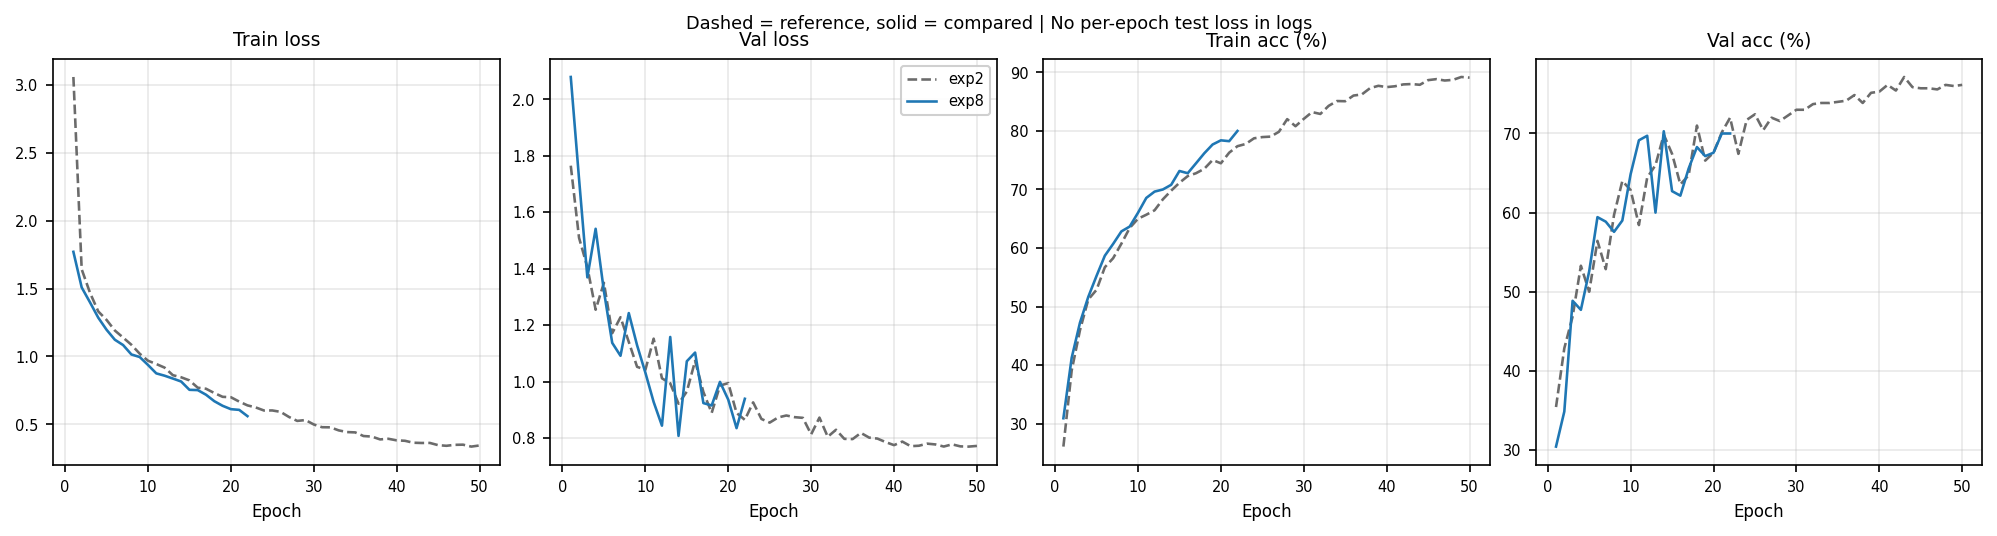
\includegraphics[width=\linewidth]{figures/comparisons/cmp_06c_exp2_exp8.png}
  \caption{exp2\_aug\_bn（虚线）与 exp8\_improved\_longer\_12（实线）}
\end{figure}

\section{可解释性分析（Grad-CAM）}
\subsection{方法说明}
Grad-CAM 用目标类别在 logits 上的标量得分对\textbf{最后一层卷积特征图}求梯度，把梯度在
空间上做一次全局平均得到每个通道的权重，再对特征图通道加权求和并取 ReLU，得到一张与
卷积特征同分辨率的类激活图，最后上采样到输入尺寸并伪彩色显示。直观上，它回答的是：
模型为了把样本判成某一类，更依赖特征图里哪些空间位置（对应到原图大致落在哪些区域）。

本实验在最后一层 \texttt{Conv2d} 上挂钩实现（未改动网络结构），热力图对应当前预测类别
的解释（即对 $\arg\max$ 类别的 Grad-CAM）。脚本使用与测试阶段一致的预处理（Resize/CenterCrop、
Normalize(0.5)）。

\subsection{可视化设置}
模型选用当前测试集表现最好的 \texttt{exp7\_improved\_long\_9} 分支对应的 checkpoint；从 STL-10 官方
划分测试集中筛选样本，分别给出\textbf{预测正确}与\textbf{预测错误}两类可视化，结果保存
在 \texttt{homework/figures/gradcam/}（含 \texttt{correct/}、\texttt{wrong/} 子目录）。
本地复现可运行：
\begin{verbatim}
python src/run_gradcam.py --checkpoint outputs_improved/exp7_improved_long_9/checkpoints/exp7_improved_long_9_best.pth
\end{verbatim}

\subsection{结果展示}
\begin{figure}[H]
\centering
\begin{subfigure}{0.48\textwidth}
  \centering
  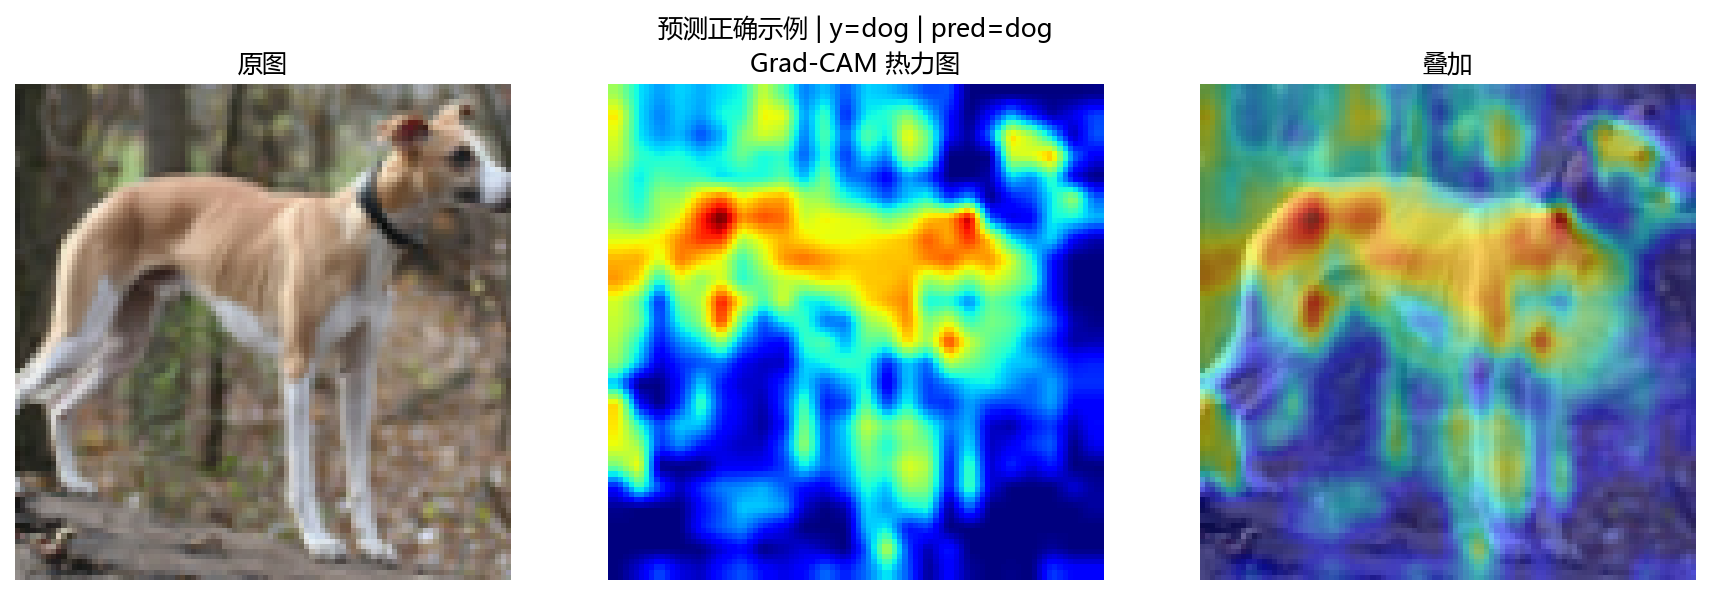
\includegraphics[width=\linewidth]{figures/gradcam/gradcam_correct_example.png}
  \caption{预测正确：热力图多集中在物体主体与轮廓附近}
\end{subfigure}
\hfill
\begin{subfigure}{0.48\textwidth}
  \centering
  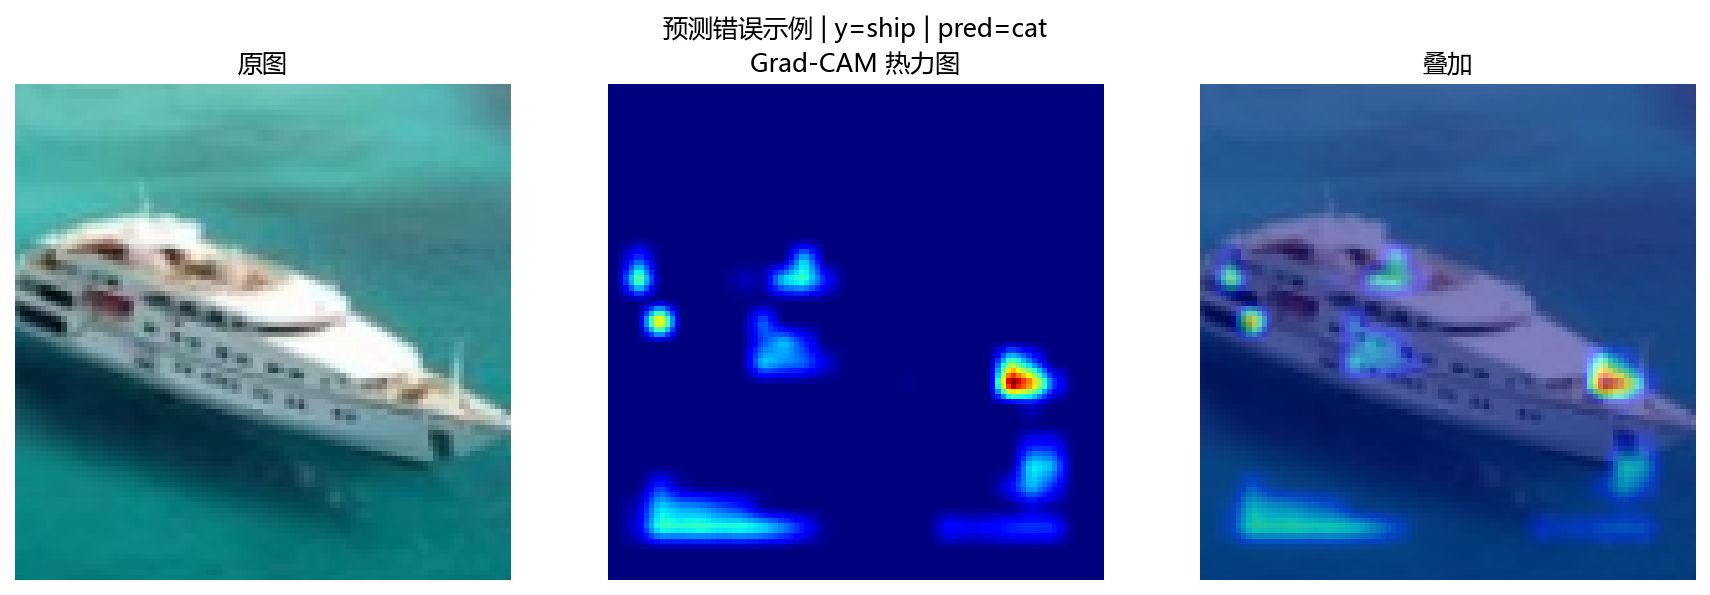
\includegraphics[width=\linewidth]{figures/gradcam/gradcam_wrong_example.png}
  \caption{预测错误：高响应区域往往偏离标签或扩散到背景}
\end{subfigure}
\caption{Grad-CAM 对比（左：正确样本；右：错误样本；均为原图/热力图/叠加）}
\end{figure}

\subsection{分析与讨论}
STL-10 图像主体相对居中、背景相对干净，若模型学到的是可迁移的语义线索，热力图应主要覆盖
物体部位而不是大片纯色背景。实验观察大致符合这一点：在预测正确的样本上，热点往往贴在物体
外轮廓与内部纹理较强区域；这与人类判断 ``物体在哪'' 的经验较为一致。

在预测错误的样本上，更容易看到两类现象：一是响应分散或偏向边缘/角落，说明模型可能被局部
噪声带走；二是热点落在与标签类别相近的部位但在细粒度上混淆（例如动物类之间），这时热力图
不一定 ``乱''，但它强调的语义区域与真实标签不一致，提示模型仍在做 ``看起来像'' 的关联，
而非完全稳健的高层语义。

\subsection{小结}
综合来看，模型并非只在像素层面做模板匹配：正确样本的可视化具有一定语义指向性；但错误样本
说明决策仍会被背景或细粒度混淆干扰，距离 ``完全可靠的高层语义理解'' 仍有差距。这与测试集
准确率约 81--82\%（\texttt{exp7} / \texttt{exp6}）相吻合。

\section{结论}
本实验完成了 STL10 图像分类任务中的 baseline 与多组优化对比。结果表明：\textbf{数据增强 + BatchNorm} 可将浅层模型推到 71.70\%；\texttt{improved\_long} 与 \texttt{improved\_longer} 等更深骨干使测试准确率最高达到 \textbf{81.60\%}（\texttt{exp7}）。\texttt{exp8\_improved\_longer\_12} 在 \texttt{exp7} 配方上继续加深至 12 个卷积层，测试仅 \textbf{69.50\%}，说明在本数据与训练预算下\textbf{并非越深越好}。\texttt{exp4}（SGD）与 \texttt{exp5}（较小 Adam lr）在固定 \texttt{exp2} 结构下未超过原 Adam 配置。

Grad-CAM 可视化进一步表明模型在多数正确样本上会关注物体区域，但错误样本仍存在背景干扰与细粒度混淆，说明模型已经学到一定语义线索，但距离完全稳健的图像理解仍有改进空间。后续可继续尝试更精细的数据增强策略、学习率调度搜索和更深层网络结构，并结合更强的可解释性方法做对照。

\section*{附件与提交说明}
按课程要求整理代码、说明文档与实验报告。可解释性脚本位于 \texttt{src/gradcam.py}（核心实现）
与 \texttt{src/run\_gradcam.py}（加载权重并导出图）。对照实验训练曲线（\texttt{cmp\_01\_baseline\_exp1.png} 等共 8 张）由 \texttt{src/plot\_comparison\_curves.py} 写入 \texttt{homework/figures/comparisons/}。运行依赖 PyTorch 与 torchvision（与训练环境一致），
数据路径默认 \texttt{STL10/}。

\end{document}
